\chapter{Probleme}
Die meisten Probleme entstanden bei der Annahme es gäbe Konsistenz in der Formatierung der Dokumente (siehe \autoref{ch:solution}, \autopageref{ch:solution}). 
\section{Dokumenttyp}
Erste Probleme tauchten noch vor der eigentlichen Extraktion auf, nämlich beim Einlesen der Plenarprotokolle in XML Form auf.
\begin{figure}[h]
	\begin{minipage}{.48\linewidth}
		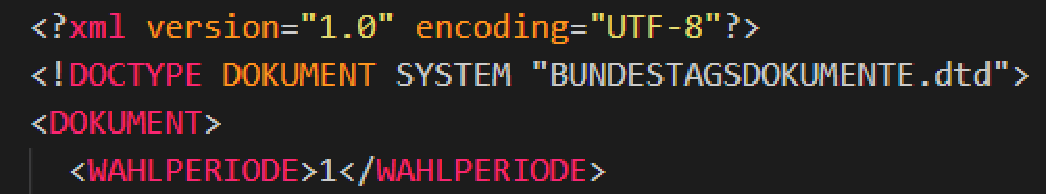
\includegraphics[width=\linewidth]{img/withdoctype.pdf}
		\caption*{Mit Angabe des Dokumententyps}
	\end{minipage}\hfill
	\begin{minipage}{.48\linewidth}
		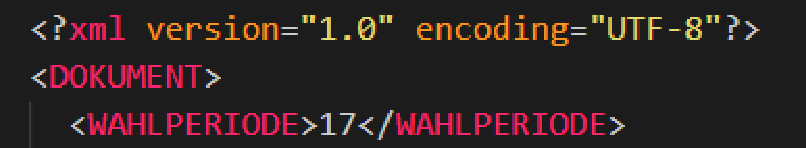
\includegraphics[width=\linewidth]{img/withoutdoctype.pdf}
		\caption*{Ohne Angabe des Dokumententyps}
	\end{minipage}
	\caption{Unterschiede in der Angabe des Dokumententyps}
	\label{img:doctype}
\end{figure}\\
In der 1. - 14. Wahllegislaturperiode wurden den XML-Dateien ein Dokumententyp angegeben, ab der 15. Wahllegislaturperiode war die nicht mehr der Fall. Beipielhaft wird dies in \autoref{img:doctype} durch ein Ausschnitt eines Protokolls der 1. und eines der 17. Wahllegislaturperiode verdeutlicht.

\section{Formatierung}
\begin{figure}[h]
	\begin{minipage}{.49\linewidth}
		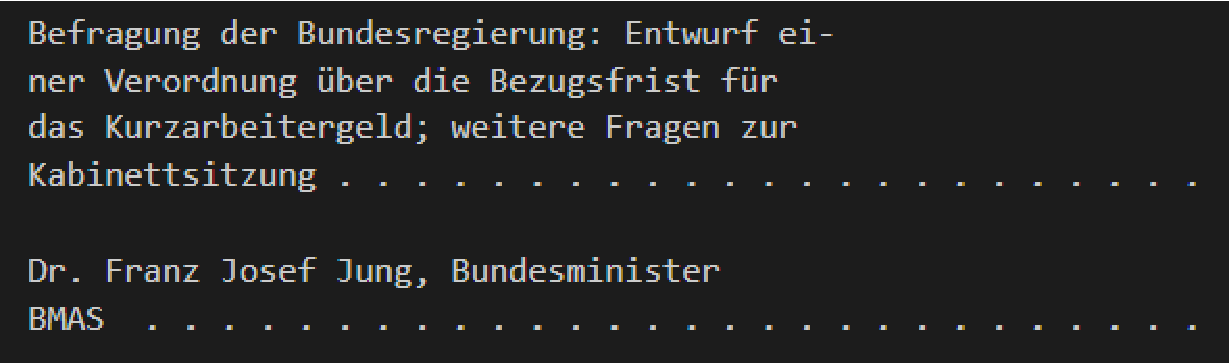
\includegraphics[width=\linewidth]{img/toc17.pdf}
	\end{minipage}\hfill
	\begin{minipage}{.49\linewidth}
		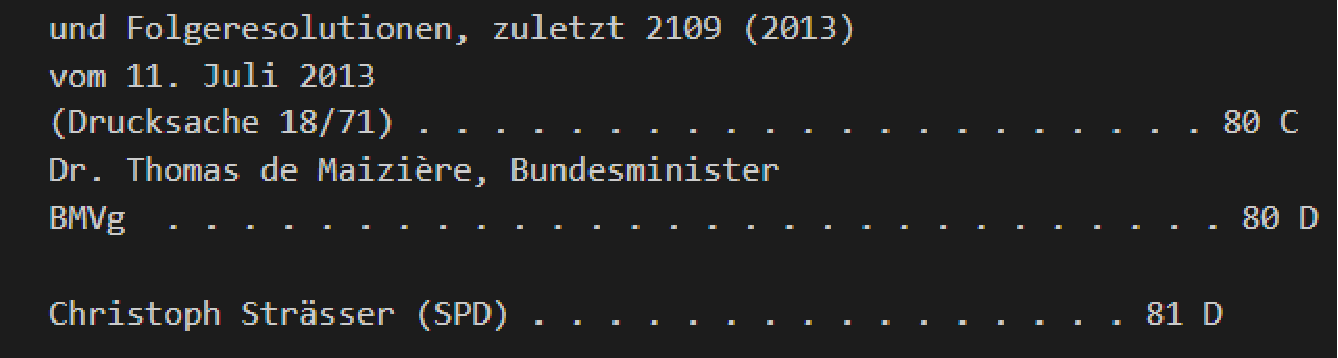
\includegraphics[width=\linewidth]{img/toc18.pdf}
	\end{minipage}
	\caption{Unterschiede in der Darstellung des Inhaltsverzeichnisses}
	\label{img:diffenzeToc}
\end{figure}

\noindent
Durch weitere Testdurchläufe wurde ein deutlicher Unterschied in den Inhaltsverzeichniseinträgen gefunden (siehe \autoref{img:diffenzeToc}), womit die Benutzung des trennenden regulären Ausdruckes nicht für alle Dokumente möglich war.  Des Weiteren ist die scheinbare Gemeinsamkeit der Punkte nicht in alle Dokumenten gegeben.\\


\section{Parteibenamung}
\Info{add hear}